\documentclass[twocolumn,10pt]{scrartcl}
\usepackage[utf8]{inputenc}
\usepackage{amsmath}
\usepackage{amssymb}
\usepackage{graphicx}
\usepackage{geometry}
\usepackage{listings, xcolor}
\usepackage{multimedia, tikz}
\usetikzlibrary{decorations.fractals}

\lstset
{
  language=C++,
  showstringspaces=false,
  captionpos=b,
  tabsize=2,
  breaklines=true,
  basicstyle=\ttfamily,
  commentstyle=\color{blue},
  stringstyle=\color{green},
  keywordstyle=\color{teal}
}
    
\geometry{hmargin=2cm,top=2cm,bottom=2.5cm}

\begin{document}

    \title{Fractal Growth \\ {\small Computational Physics}}
    \author{\small Benedikt Sauer, Alexander Schroer}
    \date{\small March 2011}

    \maketitle
 
    \section{Introduction}
        In 1981, Witten and Sander discovered that complex dendritic structures could be created by having
        `particles' perform a random walk on a lattice and stick together on contact (fig.~\ref{fig-wsdendrite}).
        This can be considered a rather surprising result, since without any preferred direction in the motion of
        particles one would naturally expect to end up with some sort of compact `blob'. In fact, structures grown
        according to this or a similar method turn out to be \emph{natural fractals}, i.e. they exhibit a certain 
        scaling behaviour within an apropriate range. The result is all the more remarkable, since Witten and Sander
        modelled it on natural phenomena -- the random walk corresponding to Brownian motion and the sticky particles
        representing some adhesive molecules or sedimenting colloids.

        The prospect that the formation of structures which had up to then been believed to be dominated by complicated
        interactions could be reduced to such easy principles together with the connection to the then just emerging
        theory of fractal geometry sparked a remarkable interest and was the basis for many follow-up publications.

        Focussing on two particular growth models developed by P.~Meakin using the results of Witten and Sander and
        M. Eden, we give a brief introduction to the basics of \emph{fractal growth}
        and present the current status of a universal toolkit capable of simulating discrete growth processes in a very
        general way. It is applied to check some earlier heurestical results.

        {\small
            \paragraph{Further reading}
                Since this text is composed in a review-like fashion and most of the information presented is
                considered to be well-known today, we will give hints for further reading at the end of each
                section instead of cluttering the text with citations.

                As for Witten and Sander's original publication and Meakin's enhancements, refer to
                \cite{src-wittensander} and \cite{src-meakin1}.
        }

        \begin{figure}
            \center
            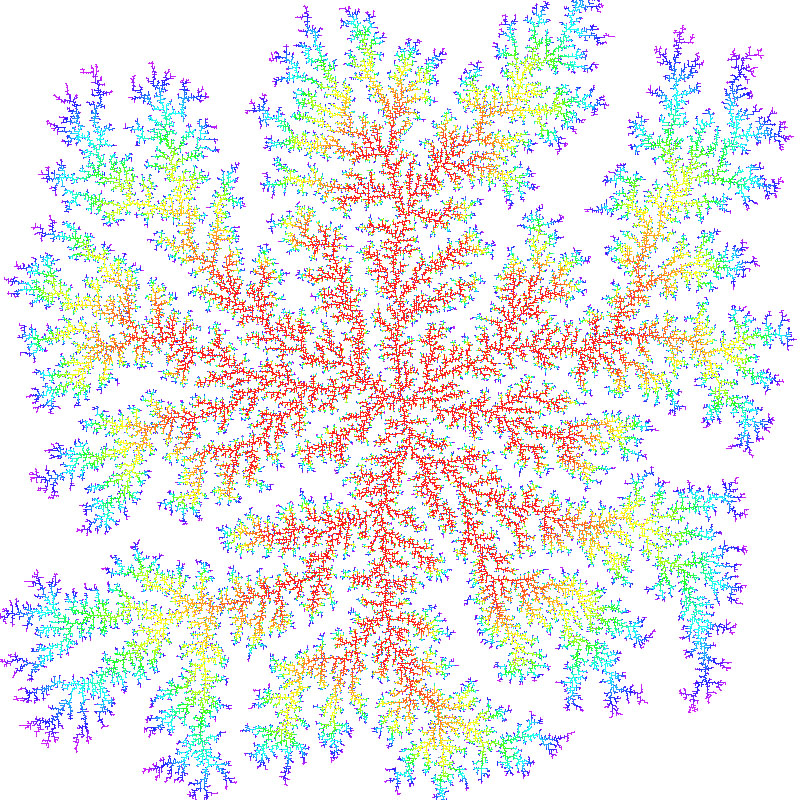
\includegraphics[width=5cm]{img/wsdendrite.jpg}
            \caption[A typical dendritic structure]
                {\small\textbf{A typical dendritic structure} grown similar to the original model of Witten
                and Sander (text). Colour-coded is the age of each particle. The cluster consists of about
                60,000 particles in total.}
            \label{fig-wsdendrite}
        \end{figure}

    \section{Some Mathematics}
        \subsection{Why talk of fractal dimensionality?}
            A possible description of geometrical objects is their treatment as subsets of $\mathbb{R}^n$, e.g. for
            three-dimensional space consider a line, a square and a cube of length, area and volume (all of which we
            will refer to as generalized volumes hereafter) 1 respectively. It is straightforward to represent the line
            by $\left[0,1\right]$ whereas $\left[0,1\right]^2$ and $\left[0,1\right]^3$ do nicely for square and cube
            -- intuitively, the volumes work out just as expected. One would now of course like to assign a 
            volume to all possible sets and can in fact do so for quite a lot -- though not for all. This idea is
            extensively treated in \emph{measure theory}.
            
            However, while volume is an important aspect to classify geometric objects we would also like to
            introduce some notion of \emph{dimensionality}. Clearly, line, square and cube should be of dimension 1, 2
            and 3. For our example this can easily be achieved (up to the border) by resorting to topology and
            basically identify a set with a manifold which is locally equivalent to a vector space
            $\mathbb{R}^m$, where $m<n$, and call $m$ the dimension of the set. Manifolds, while having a great deal
            of interesting properties, are hardly a typical example of arbitrary subsets of $\mathbb{R}^n$, though.
            
            A more general approach, which works for any topological (sub-)space and thus trivially for any open subset
            of $\mathbb{R}^n$, is given by the \emph{Lebesgue covering dimension}: If always some points of the set are
            contained in at least $n+1$ elements of an arbitrarily fine open cover, the set is of dimension $n$.

            There is a bunch of other (non-equivalent) approaches to assign sets an integer which is called
            \emph{dimension} and coincides with what one would expect for our examples and other `everyday objects'.
            However, at some point, quite another issue arises. As an example, consider the \emph{Koch curve}
            (fig.~\ref{fig-koch}), which starting with the interval $\left[0,1\right]\subset\mathbb{R}^2$ can be
            constructed as follows:

            \begin{itemize}
                \item divide the interval into three parts of equal length,
                \item replace the middle part by two parts of the same length which together with the removed part
                    form an equilateral triangle,
                \item repeat these steps for each of the smaller parts.
            \end{itemize}

            The catch is this -- what dimension do you \emph{want} to assign to this set? It should probably be
            one dimensional. After all, has been constructed from lines. But than again, its length is infinite
            (precisely $\lim_{n\rightarrow\infty}\left(\frac{4}{3}\right)^n$) whilst its extent is finite. Surely, such
            an object should cover some finite area? Unfortunately, the Koch curve being two-dimensional is clearly
            ruled out by our topological definition. In fact, the topological dimension of the Koch curve can easily be
            verified to be 1, which seems somewhat unfitting.

            The Koch curve is just an example of many sets which can be defined using a so-called
            \emph{iterated function system}: Given a set of affine
            functions which are contractive on the average, the set of points which is invariant under the action
            of the functions has similiar properties as the Koch curve. Another famous set which can be constructed by
            an IFS is the Sierpinski triangle (fig.~\ref{fig-sierpinski}).

            Alternatively, consider an infinite random walk in two dimensions. The resulting path is one dimensional by
            construction, but since every point in space has a finite probability of being reached, after an infinite
            number of steps, the whole space should be covered. So is the path one- or two-dimensional?

            It turns out that it is a fruitful idea to resort the obvious, though unintuitive solution: define
            fractional dimensions. By constructions which will be discussed in a second, one can assign the dimensions
            1.26, 1.58, and 1.33 to the Koch curve, the Sierpinski triangle and the
            random walk respectively. They all are embedded in two-dimensional space, so their dimension has to be
            less than or equal to 2, and their topological dimension is 1, which serves as a lower boundary.

            Structures of non-integer dimension are called \emph{fractals}.

        \subsection{The fractal (Hausdorff) dimension}
            One can put these observations on a firm mathematical footing by introducing the outer Hausdorff measure

            \begin{equation*}
                H^d_\varepsilon(S)=
                \inf_{\substack{\bigcup_{i=1}^\infty U_i\supset S\\ \operatorname{diam}(U_i) <
                \varepsilon}}
                    \sum_{i=1}^\infty \operatorname{diam}(U_i)^d
            \end{equation*}

            and define the Hausdorff dimension for a measurable set $S$ as

            \begin{equation*}
                d_H = \sup\{d\in\mathbb{R}^+_0\ |\ H^d(S) = \infty\}.
            \end{equation*}

            While this looks rather intimidating at first sight, it boils down to the same idea which was behind the
            covering dimension, although being much more versatile and applicable to any set with a well-defined
            volume, which includes some rather pathological cases. Again, this is dealt with in greater detail in
            measure theory.

            Fortunately, in well-behaved cases there is an easy implication. Note that we will not define the precise
            meaning of `well-behaved'. In general, however, fractals which can be constructed explicitely, e.g. by
            an IFS, tend to be `well-behaved'. The implication is this: Connected to the dimensionality of a set
            is a certain scaling behaviour concerning the number $N$ of spheres of radius $R$ covering the set, namely
            for $R\rightarrow 0$, $N\propto R^{-d_H}$. While this is just a reformulation of what we have already had
            before (provided spheres are suited as covering sets), writing it this way allows for further modification
            to yield a very useful expression:

            \begin{equation}
                d_H=-\lim_{R\rightarrow 0}\frac{\log N}{\log R}.
                \label{eq-bcdimlim}
            \end{equation}

            By this, you can easily confirm, that indeed, the dimension of the Koch curve is
            $\frac{\log{4}}{\log{3}}\approx 1.26$. The expected results for geometric primitives are also easily
            recoverable.

            This scaling behaviour can be viewed as an illustration for the connection between fractal dimensionality
            and \emph{self-similarity}. Self-similarity is a striking aspect of fractals and describes the fact that
            viewed on different scales, fractals look essentially the same. In the case of IFS fractals this similarity
            is exact. But there are as well true fractals with only approximate self-similarity, the most famous
            example probably being the Mandelbrot set.

        \subsection{Improper fractals}
            Up to now he have only talked about sets the construction of which involved some limiting procedure. This
            is clearly not apt to describe natural phenomana which are always limited and finite. Nevertheless, when
            looking at the right scale, fractal characteristics may emerge. In terms of the example of dendritic growth
            discussed in the introduction, clearly it is neither useful to study the structure at the atomic scale,
            nor at a macroscopic one. But a a certain \emph{mesoscopic} scale, the dendritic structure exhibits a large
            amount of self-similiarity (fig.~\ref{fig-selfsim}). Our immidiate aim therefore is to further generalize
            our notion of fractal dimensionality to encompass these kinds of structures as well.
            
            We can do so in a somewhat ad-hoc fashion: Again consider the minimal number of spheres of radius $R$,
            $N(R)$, required to cover the structure. But now, instead of taking the limit of a small radius, define the
            fractal dimension $d$ at the scale given by $R$ as

            \begin{equation}
                d(R)=-\frac{\log N(R)}{\log R}.
                \label{eq-bcdim}
            \end{equation}

            Note that this is almost identical to eq.~\ref{eq-bcdimlim}. 
            The value of $d$ obtained by this conecpt is called \emph{box-counting dimension} and it does not
            neccessarily equal the Hausdorff dimension. In fact, in most cases it does not -- remember, we are not
            talking about true fractals any longer. $d$ becomes a meaningful quantity if it does
            not change (much) over the scales under consideration. This information is usually extracted from
            log-log-plots (fig.~\ref{fig-scale}).

            There are also other ways to determine the fractal dimension from scaling laws. In fact, one should rather
            call them methods to find a (sic) fractal dimension, because just as with box-counting and Hausdorff,
            equivalences break down due to finite-size effects. Then again, there are some scaling laws which give
            approximately the right dimensionality (i.e. in accordance to other established recipies) for no good
            reason at all.
            
            Two methods which are often applied in $\mathbb{R}^n$ with Lebesgue metric and which will be particularly
            suited to our ends are
            \begin{itemize}
                \item $R_\mathrm{gyr}\propto m^{1/d_H}$,\\where $R_\mathrm{gyr}=\frac{1}{m}\left(\int_V \mathrm{d}^n x
                    \rho\left(x\right)\left(x-x_0\right)^2\right)^\frac{1}{2}$ is the radius of gyration around the
                    center of mass $x_0$, $V$ the volume and $m=\int_V \rho$ the mass and
                \item $C(r)\propto r^{D-d}$,\\where $C(r)=\rho\star\rho$ is the density-density correlation.
            \end{itemize}

            The density $\rho(x)$ is usually defined as 1 if $x$ belongs to the fractal and 0 else.

            Structures which exhibit a fractal-like scaling behaviour over certain ranges are common in nature. Typical
            examples include coast lines, veins and cracks.

        {\small
            \paragraph{Further reading}
            The rough sketches of topology and measure theory can be reviewed in any decent book on advanced analysis.
            For a comprehensive introduction to fractal geometry, have a look at \cite{src-mandelbrot}. Different
            methods to measure the fractal dimension of finite structures can be found e.g. in \cite{src-stanley} and
            \cite{src-wittensander}.
        }

        \begin{figure}
            \center
            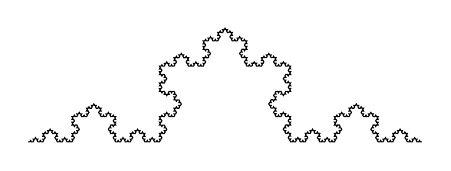
\begin{tikzpicture}[decoration=Koch snowflake]
                \draw decorate { decorate { decorate { decorate { decorate { (0,0) -- (5,0) }}}}};
            \end{tikzpicture}
            \caption[The Koch curve]
                {\small\textbf{The Koch curve} is a well-known example for a fractal structure ($d_H=\frac{\log 4}
                    {\log 3}$)}
            \label{fig-koch}
        \end{figure}

        \begin{figure}
            \center
            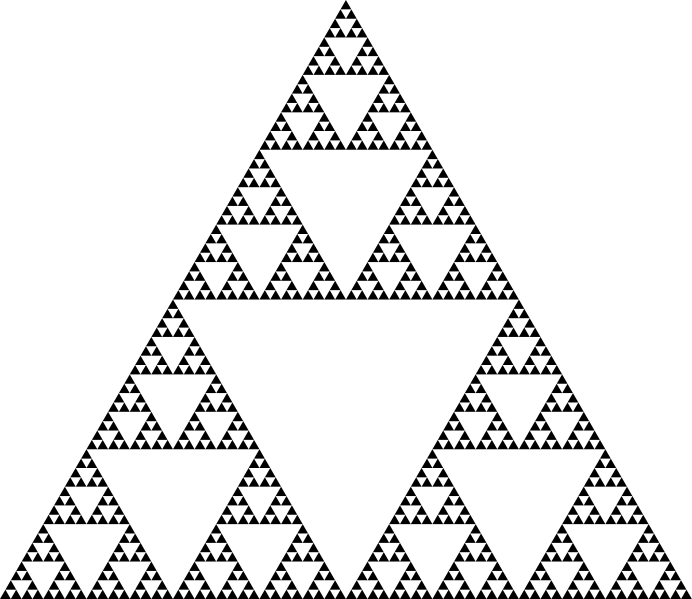
\includegraphics[width=5cm]{img/sierpinski.png}
            \caption[The Sierpinski triangle]
                {\small\textbf{The Sierpinski triangle} is another famous example for a strictly self-similar fractal
                which can be defined as the solution of an iterated function system. Wikimedia Commons.}
            \label{fig-sierpinski}
        \end{figure}

        \begin{figure}
            \center
            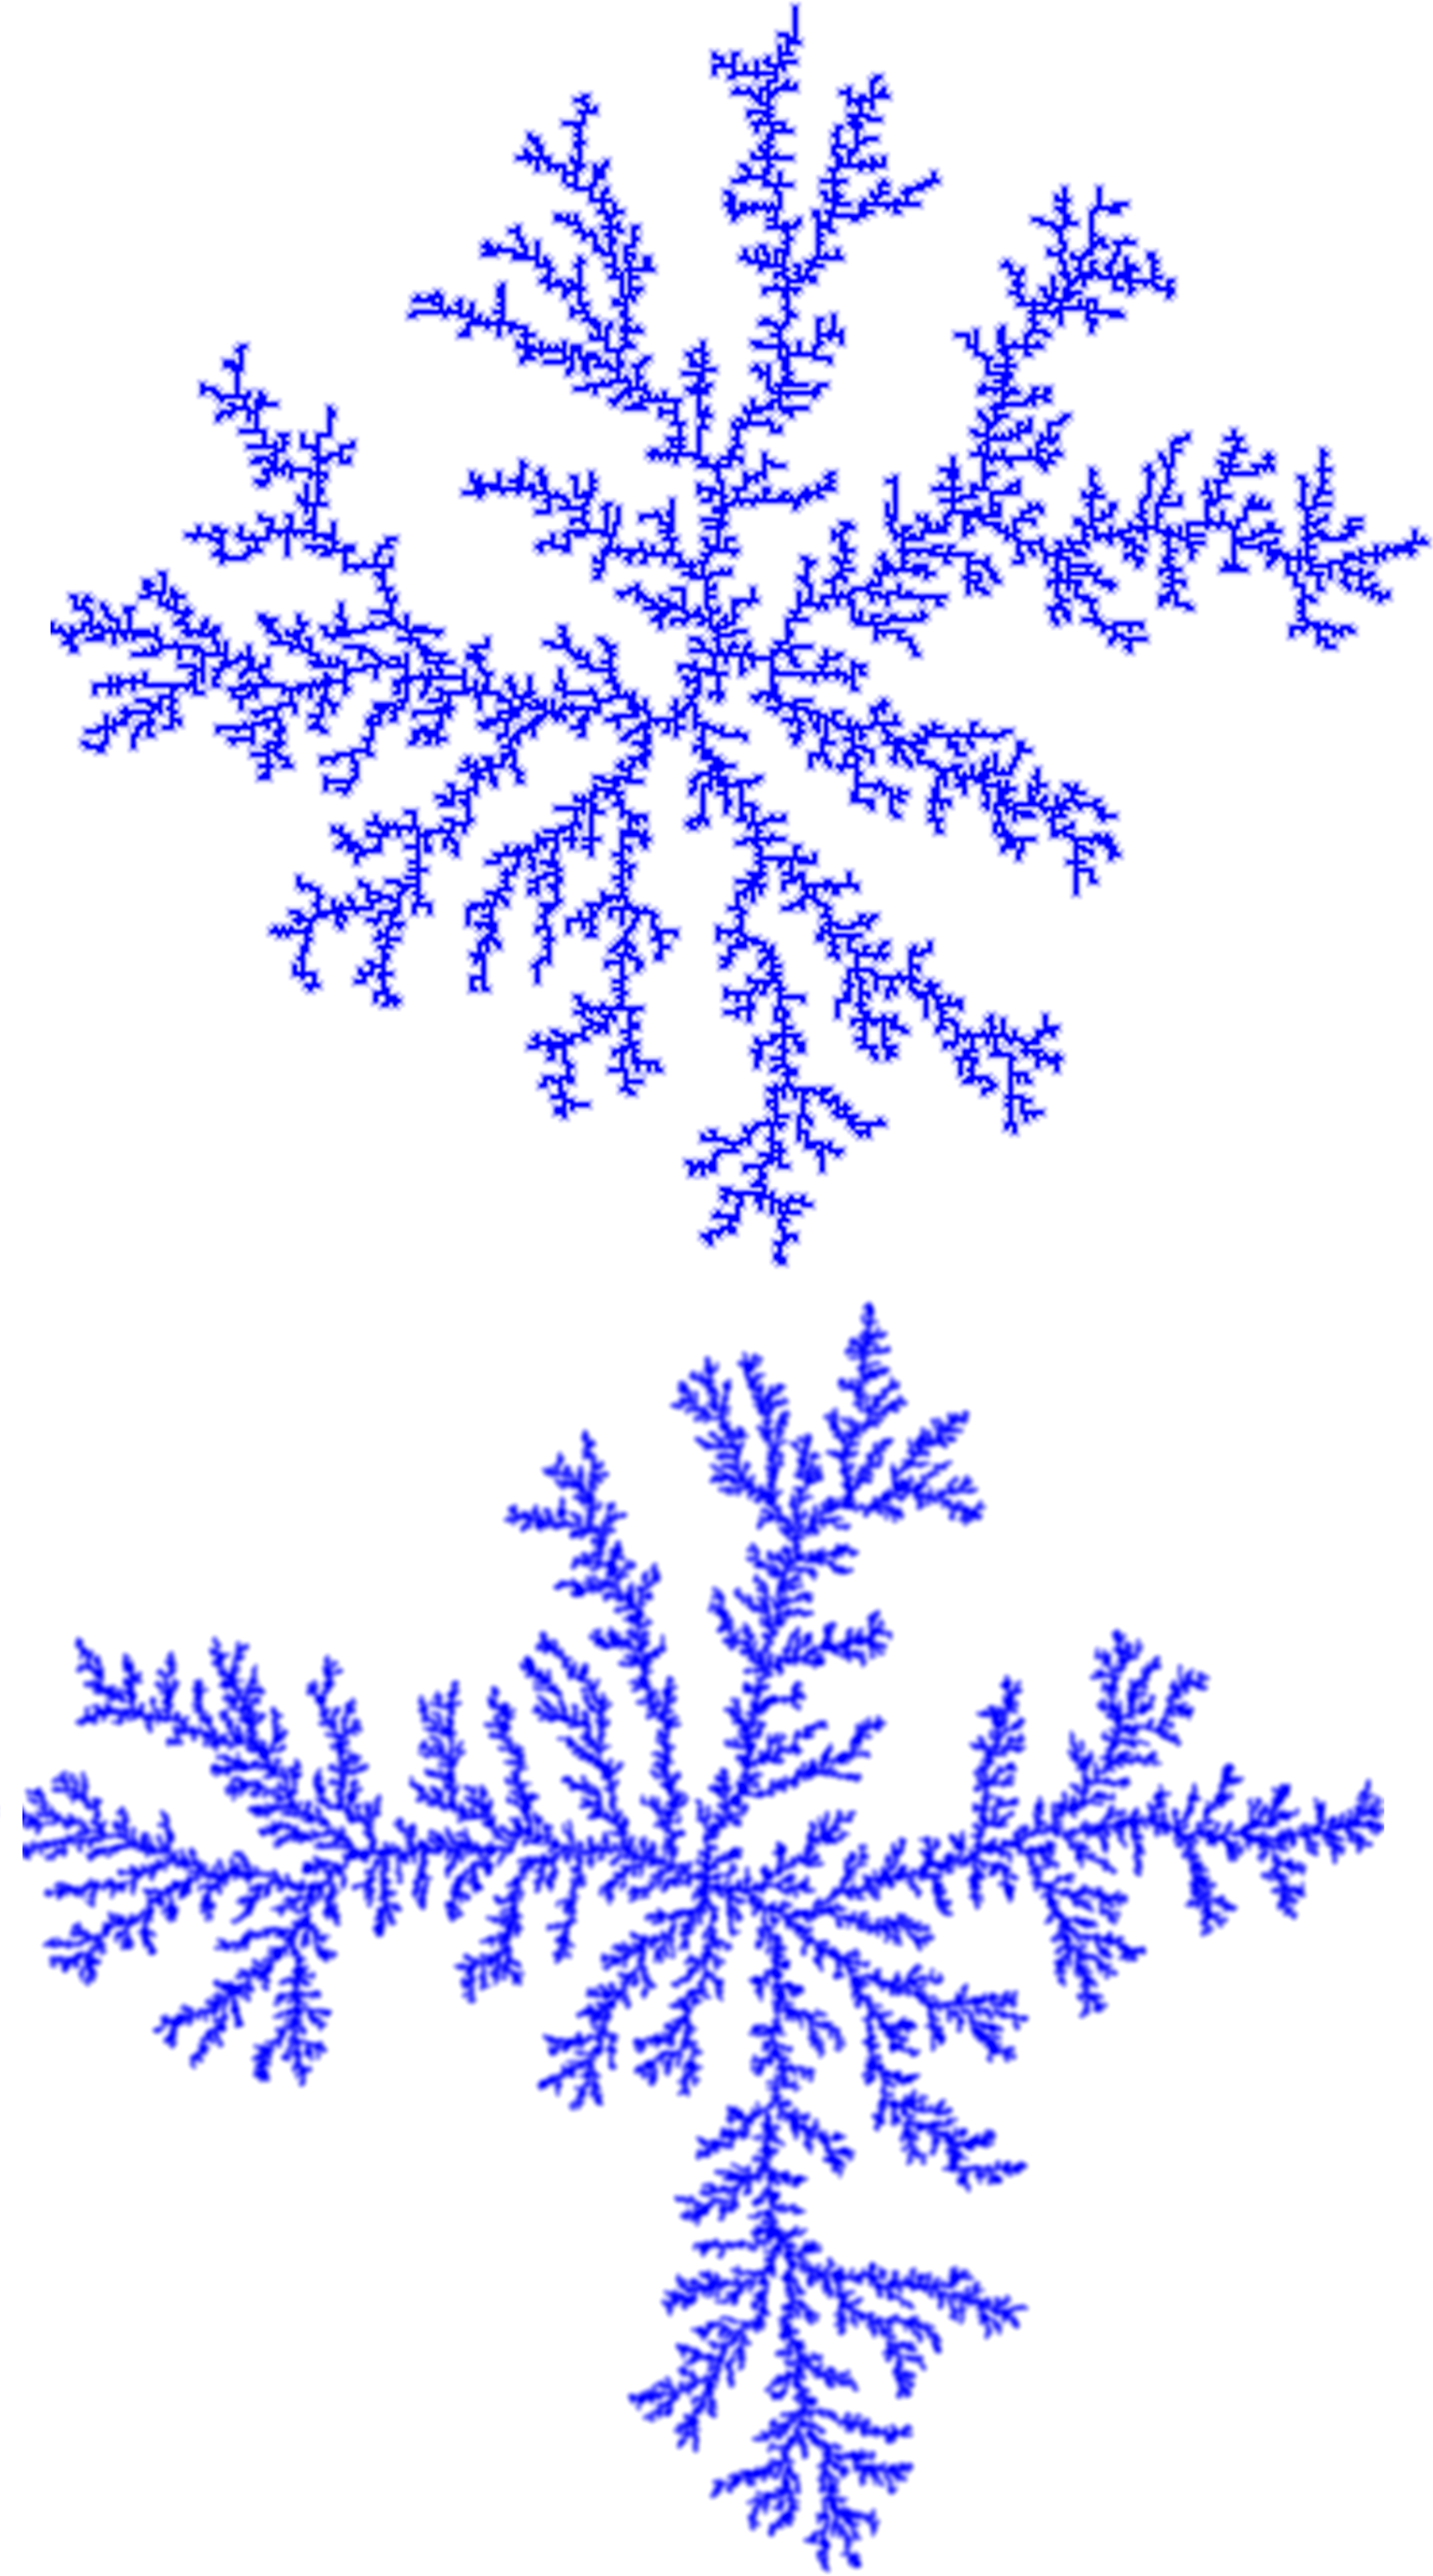
\includegraphics[width=5cm]{img/selfsim.png}
            \caption[Self-similarity]
                {\small\textbf{Self-similarity} is a form a scale invariance. The upper cluster consists of 10,000
                particles, whereas the lower one contains 100,000 particles. Note that the larger cluster just appears
                to have a slightly more detailled boundary. Actually, it has grown much larger; the size of the
                individual particles is unchanged.}
            \label{fig-selfsim}
        \end{figure}

        \begin{figure}
            \center
            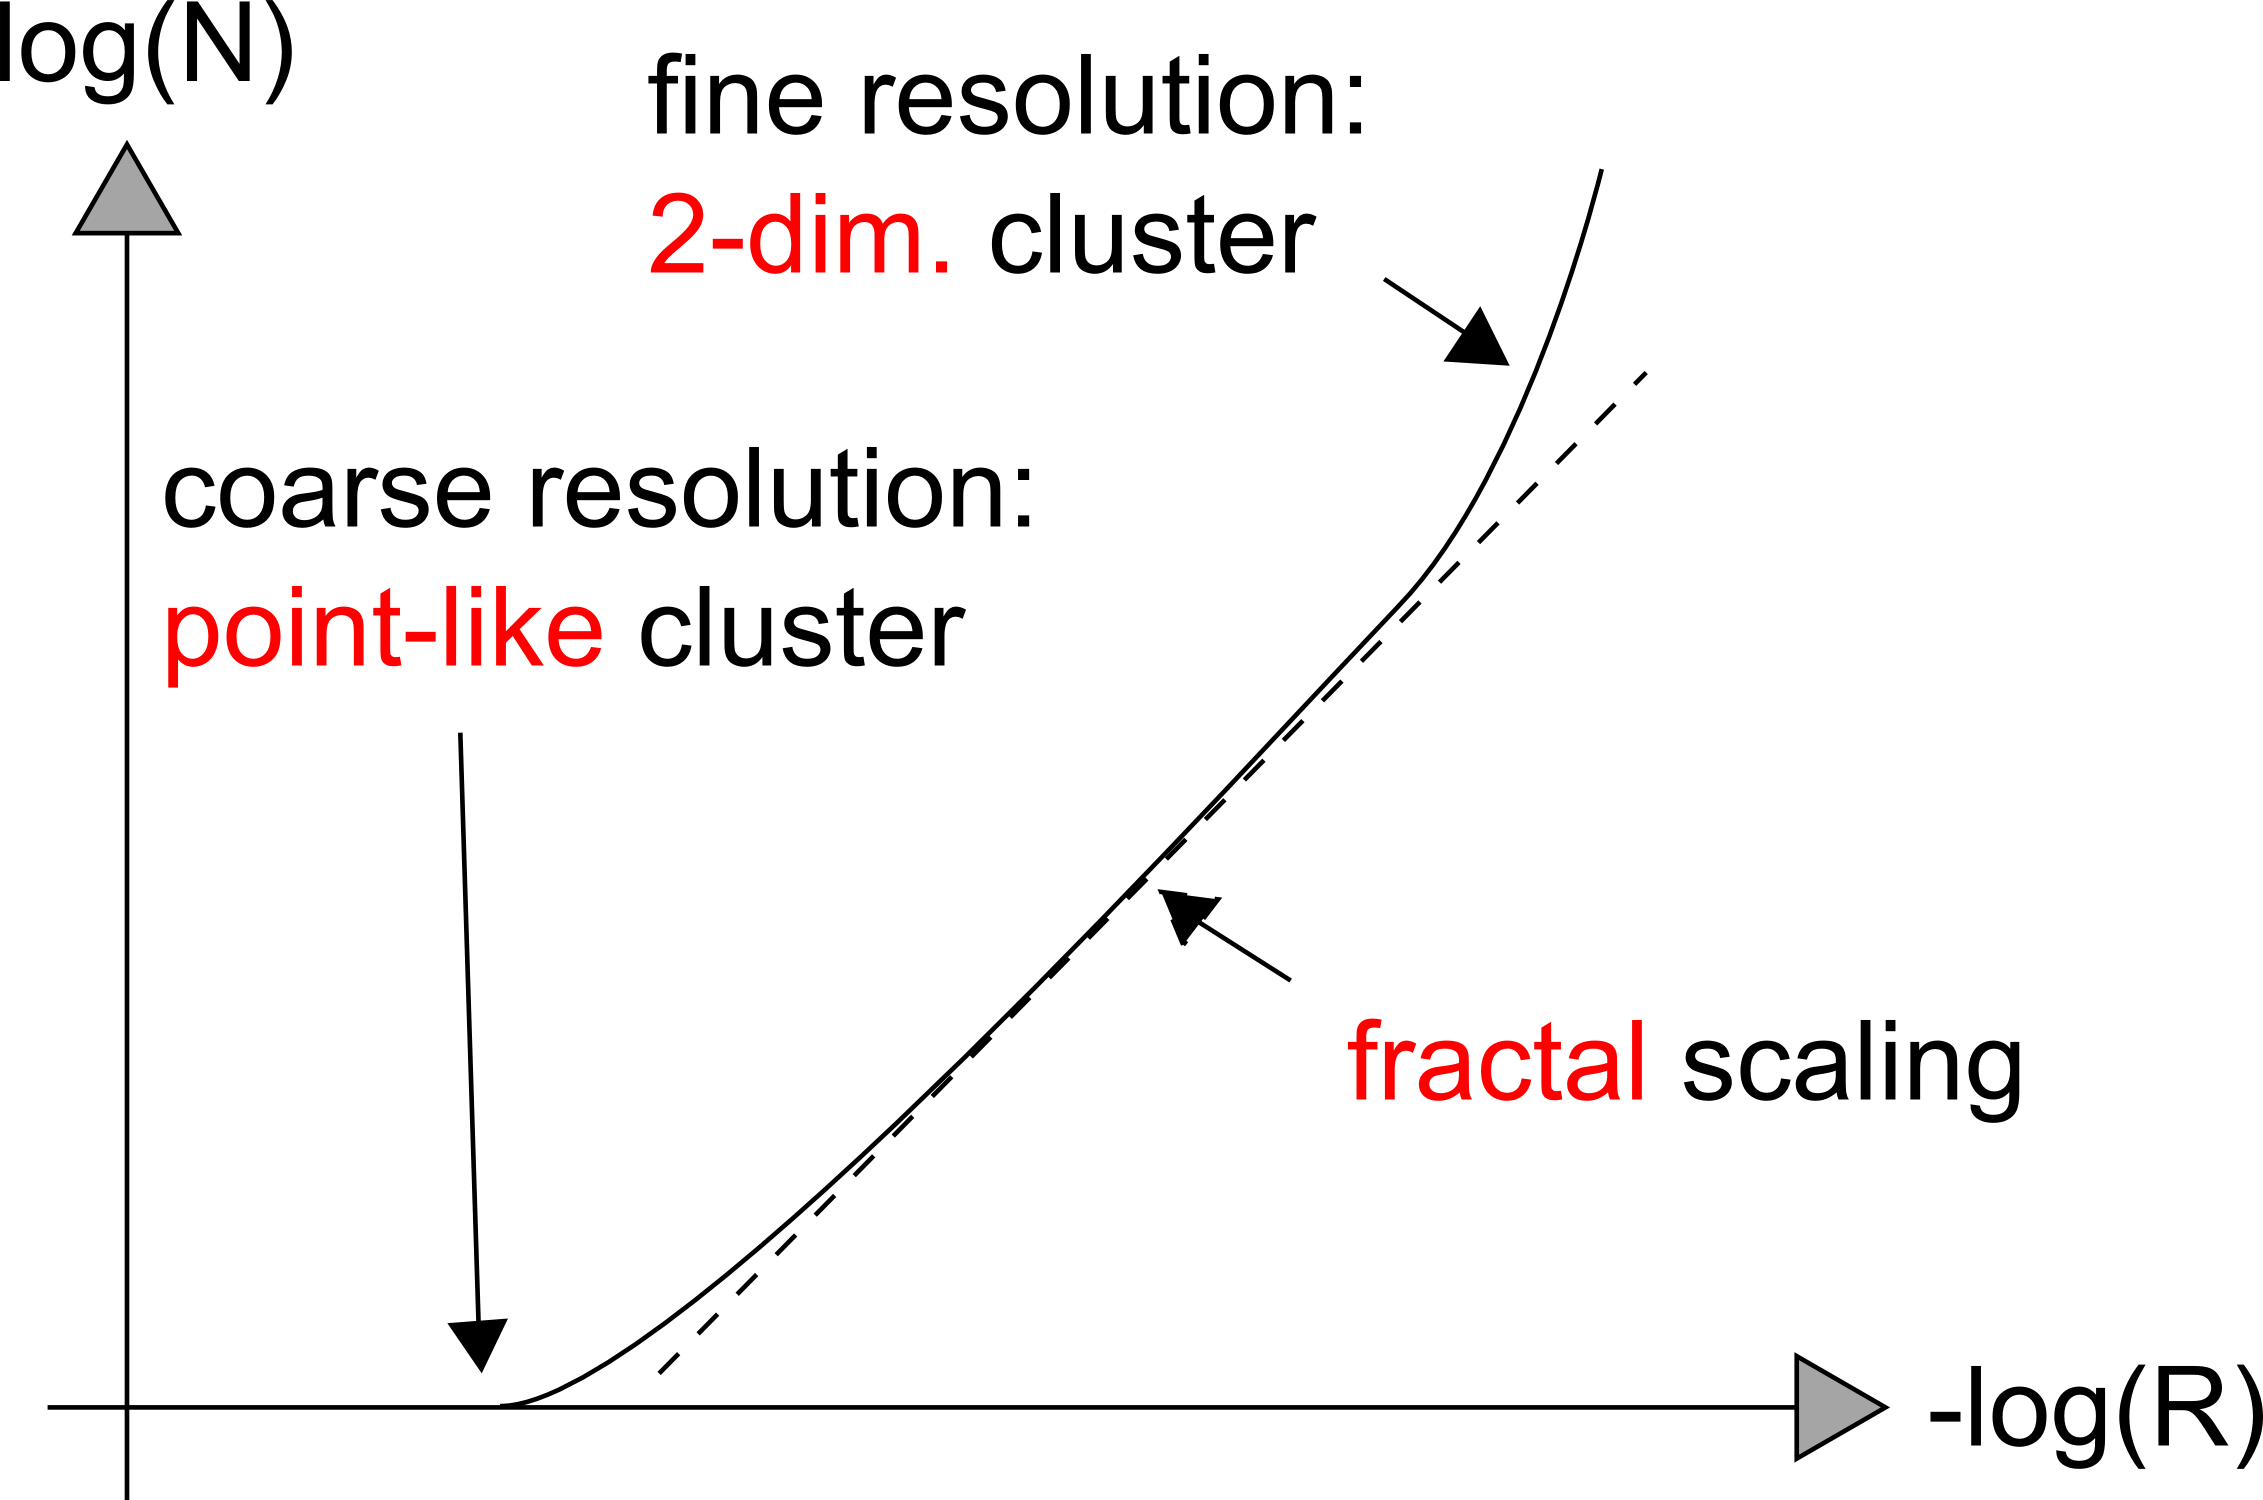
\includegraphics[width=5cm]{img/scale.png}
            \caption[Improper fractals]
                {\small\textbf{Improper fractals} exhibit fractal scaling behaviour only over a certain range.
                In this example, the fractal is composed of two-dimsensional objects and has a finite size
                which induces different scaling behaviours at large and small scales.}
            \label{fig-scale}
        \end{figure}

    \section{The Meakin model}
        The Meakin model comprises two aspects: \emph{diffusion limited aggregation} and \emph{number limited
        aggregation}. Both deal with particles perfoming a random walk and stick together on contact just like
        Witten and Sander proposed. In the case of \emph{diffusion limited aggregation} (DLA), one follows the
        pattern
        \begin{enumerate}
            \item create a single particle at the origin and call it the cluster (seeding);
            \item create a new particle at a random position, uniformly chosen on the n-sphere with radius
                $r=r_\mathrm{C}+10$ particle diameters around the unweighted center of the cluster.
                $r_\mathrm{C}$ labels the `cluster radius', which
                is defined as the minimum radius of an n-sphere which completely contains the whole cluster;
            \item let the new particle perform a random walk. It becomes part of the cluster in the instant
                they touch;
            \item go back to step 2.
        \end{enumerate}
        Creating particles shortly beyond the cluster radius simulates diffusion from infinite distance, simply
        because at some point, that boundary has to be crossed. Outside this region, the influence of the
        internal structure of the cluster on the random walk trajectory is assumed to be negligible. To speed things up,
        particles have to be removed again if they wander to far from the cluster. Usually, a distance of
        $2r_\mathrm{C}$ from the center of the cluster is chosen as a border beyond which particles are removed
        and a new one is created. This is discussed in more detail in the section on the implementation.
       
        One of Meakin's most important results is that the model can be maximally discretized without changing
        its properties. Here, maximum discretization means to perform the random walk on a lattice with
        a lattice spacing equal to the particle diameter. Two particles can be considered to be touching if
        they are located at nearst-neighbour lattice sites. Moreover, the particular choice of a lattice does
        not have measurable effects either. Therefore, all simulations can be performed on n-dimensional
        cubic lattices, which obviously is a huge advantage from the implementation point of view.

        Meakin investigated the fractal dimension for embedding dimensions $D=2$ to 6, mainly via radius of gyration
        and density-density-correlation, and came to the conclusion that very roughly $d_H=\frac{5}{6}D$.
        On a qualitative level, the resulting structures are approximately spherical and strongly dendritic,
        much like patterns of ice on a window. They can be seen in fig.~\ref{fig-selfsim}.

        \emph{Number limited aggregation} consists of the following steps
        \begin{enumerate}
            \item create a given number of particles on a lattice with periodic boundary conditions;
            \item particles which touch are joined to clusters;
            \item particles which touch clusters are added to them;
            \item cluster which touch are merged;
            \item move all particles and clusters randomly;
            \item go back to step 2.
        \end{enumerate}
        Optionally, clusters have a certain probability not to move which is proportional to the number of
        particles they consist of, thereby simulating `mass'. This results in net-like structures
        (fig.~\ref{fig-meakin2}) with a fractal dimension of about 1.5 in 2-dimensional embedding space. Again, Meakin
        could not find discretization artifacts caused by the lattice.

        {\small
            \paragraph{Further reading}
            Meakin's models are presented in \cite{src-meakin1} and \cite{src-meakin2}.
        }

        \begin{figure}
            \center
            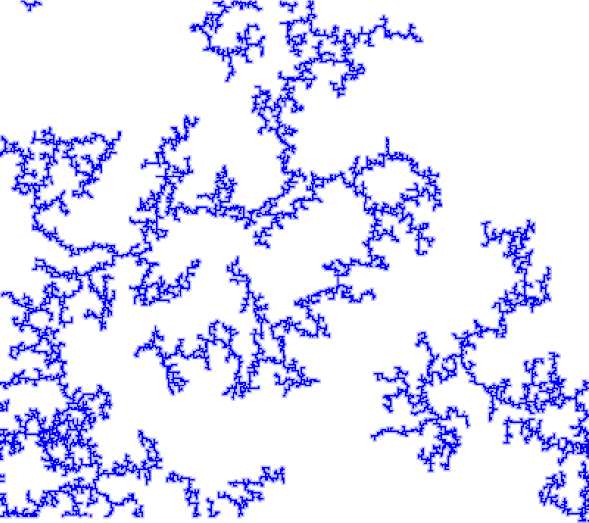
\includegraphics[width=6cm]{img/meakin2.png}
            \caption[Number limited growth]
                {\small\textbf{Number limited growth} with 16,000 particles on a 2-dimensional 400x400 lattice.}
            \label{fig-meakin2}
        \end{figure}

    \section{The Eden-Meakin model}
        In contrast to the Meakin-model discussed before, the Eden-Meakin model is inspired by organic rather than
        anorganic processes. In 1961, M. Eden investigated the following growth model on a lattice:
        \begin{enumerate}
            \item start with a single particle;
            \item add a particle at a random lattice site with a probability proportional to the number of its
                occupied neighbours;
            \item go back to step 2.
        \end{enumerate}
        Unsurprisingly, what forms very much looks like a cell culture or a fungus. Eden asked the question:
        To what extend do random effects influence the development of biologic systems? Rephrased in a fancy
        way this is: Why do monozygotic twins have different finger prints? Eden's approach was purely analytic
        (or combinatoric); he did some simulations, though rather as a last resort and without much enthusiasm.
        But then again, this was in 1961. When Meakin build his model of adaptive growth on top of Eden's model
        in 1991, he took a purely numeric approach instead. The boundary of Eden's cell culture had already
        been discovered to have a fractal dimension, but Meakin was interested in something different: He
        introduced a scoring system to determine, which cells (particles) are `important' for the whole cluster
        and remove the irrelevant ones. This works as follows:
        \begin{itemize}
            \item whenever a new particle is added, assign it an initial score of 0 and a `parent', which is
                one of its neighbours (e.g. the one with the highest score or a random choice),
            \item the new particle and all of its ancestors (forming a unique chain back to the seed of the
                cluster) are awarded a score $\Delta S=(1+l)^{-\eta}$, where $l$ is the length of the chain
                and $\eta\in\mathbb{R}_+$ is a parameter,
            \item reduce the score of each particle in the cluster by $\frac{1}{N_m}$, $N_m\in\mathbb{N}$,
                and remove particles of negative score.
        \end{itemize}
        Amazingly, a dendritic backbone of high-scored particles develops (fig.~\ref{fig-eden}), which has a
        fractal dimension,
        the exact value of which depends on the cut-off score. There are other properties, however, which
        might be considered even more interesting.

        First of all, the cluster only reaches a finite size. This is conceivable, because the larger it
        becomes, the more possibilities there are to add new particles and the smaller is the score a new
        particle is initially assigned. Therefore, new particles will be removed before they become parents
        to another particle themselves. Meakin gives a crude but easy estimate about the final size depending on
        $\eta$ and $N_m$ in his publication.

        Secondly, the model is adaptive. The meaning of this can most easily be demonstrated by an example.
        Fig.~\ref{fig-edenadap} shows the number of particles in two clusters grown with different parameters.
        At the time marked by the vertical bar, the parameter sets are swapped. Soon after, the cluster
        sizes have swapped as well, thus adapting to the new conditions. This stands in clear contrast to the
        strictly irreversible growth models discussed so far.

        Third, the cluster has a memory. It can also be seen from fig.~\ref{fig-edenadap} that the total score
        of the clusters keeps on growing all the time. Because most of it is alotted to the backbone, it
        takes an increasingly large number of steps to remove a particle from it, once conditions change.
        Another way to say this is that as parts of the cluster become older, they become less adaptive as well.

        We can therefore safely state that the Eden-Meakin model has not only been \emph{inspired} organically
        but also exhibits behaviour commonly attributed to living entities.

        {\small
            \paragraph{Further reading}
            The original model as presented by M. Eden in 1961 is \cite{src-eden}. Meakin's modifications are
            covered in \cite{src-meakin-eden}.
        }

        \begin{figure}
            \center
            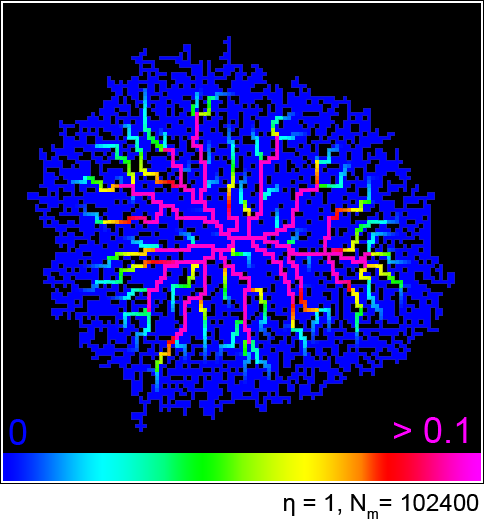
\includegraphics[width=5cm]{img/eden.png}
            \caption[The Eden-Meakin model]
                {\small\textbf{The Eden-Meakin model} produces different dendritic structures depending on the
                cut off-score (colour-coded).}
            \label{fig-eden}
        \end{figure}

        \begin{figure}
            \center
            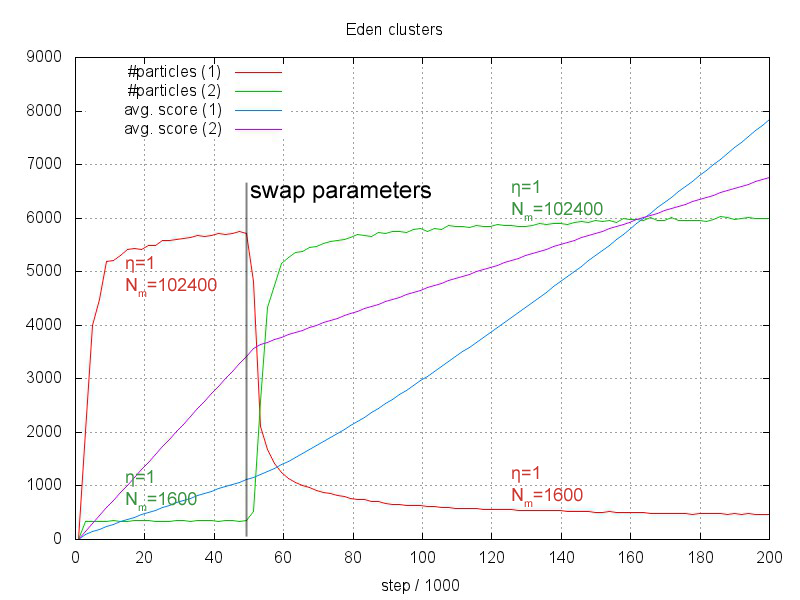
\includegraphics[width=7cm]{img/edenadap.png}
            \caption[The adaptive nature of the Eden-Meakin model]
                {\small\textbf{The adaptive nature of the Eden-Meakin model} can be seen, if two clusters are
                grown with different parameter sets. If the parameter sets are exchanged, the cluster sizes
                swap as well. The total score increases monotonically. This renders the cluster more passive
                towards changed over time and can be interpreted as a memory.}
            \label{fig-edenadap}
        \end{figure}

    \section{\lstinline!trivial! -- a fractal growth toolkit}
        To implement the models described above we designed a generic C++ toolkit to 
        In our implementation we tried to focus on the following design goals, using object-oriented techniques:
        \begin{description}
            \item[Performance] We have to make multiple runs to get sufficient statistics, so it is important that the
                programs generate large clusters in short times.
            \item[Genericness] Because the models we are implementing are very similar it would be nice from a
                programmer's point of view to have one basic implementation with pluggable components. Also we wanted to
                implement every model for every possible (metric) topology (dimension, boundary conditions, etc.)
                exactly once.
        \end{description}
        To unify both goals (which are actually quite contrary) we heavily relied on C++ templates. With a decent
        compiler (we used the current G++, version 4.5.2) this gives us the performance of hand-written C or C++ code
        (which we tried out first), while remaining very versatile. The library is still under development and we are
        going to implement some major changes described in the last section in the near future to make it even more
        useful.

        In its current state the toolkit allows us to implement the basic models described before in arbitrary
        dimensionalities with 2 and 3-dimensional (anaglyphic) real-time visualization, extraction of statistical
        information during the growth, and drawing of single images of 2-dimensional clusters. We can also plug in
        arbitrary random number generators, where in our calculations we always used the Mersenne Twister (MT 19937, see
        \cite{src-matsumoto}).  Number limited growth calculation in higher dimensionalities than 2 is not mentioned in
        any of the papers we read but is also possible with \lstinline'trivial'.

        Furthermore we have implemented some optimisations especially for the Meakin model
        TODO
        
        The toolkit also enabled us to experiment with different setups, detailed in the last part of this section,
        which increases its practical use.

        %any dimension, ultra-fast, versatile, building-block approach, still under development, mt13397,
        %no different step sizes, ability to do meakin2 in any dimension etc (not mentioned elsewhere)
        %visualization

        \subsection{Details on the implementation}
            %kill-radius, cluster/particle types, multiindex, templates, radius for collision checks, n-sphere,
            %periodic boundary conditions
            A typical \lstinline'trivial'-program currently looks as follows:
            \begin{lstlisting}
typedef meakin::sticky_particle<position<3>> particle_type;
typedef meakin::static_cluster<particle_type> cluster_type;
typedef meakin::diffusion_limited_updater<particle_type, cluster_type> updater_type;
typedef world<particle_type, cluster_type, updater_type> world_type;

gl_visitor<world_type> visitor;
world_type w;

for (int n = 0; n < 1e6; ++n)
{
    w.step();
    if (n % 100 == 0)
        w.accept(visitor);
}
            \end{lstlisting}
            This implements a diffusion limited growth of a single static cluster in 3 dimensions which is visualised
            using OpenGL every hundredth step and terminates after the millionth.

            As one can see from this, there are four major building blocks in our program:
            \begin{enumerate}
                \item The \lstinline'world' Template
                \item The particle type
                \item The cluster type
                \item The updater type
            \end{enumerate}
            Additionally there is the position type that completely defines our metric topology and is in this case just
            a 4-dimensional vector, and the visitor interface that allows us to get the current state of the world (here
            only to provide some visualisation, in actual programs maybe for statistics or loading and saving states).

            In the following we'll look into the concepts of those building blocks and describe some of their provided
            implementations.

            \subsubsection{The \lstinline!world! Template}
                This template class is the main interface to the toolkit. It has four template parameters, the basic
                \lstinline!Particle! type it should use, the type of \lstinline!cluster!s that get created when
                particles merge, and the \lstinline!Updater! type, which handles creation and destruction of objects in
                each step.  Additionally the type of the \lstinline!RandomNumberGenerator!, which defaults to a Mersenne
                Twister in our case, is parametrized, which allows us to use different (i.e.\ faster) generators if
                necessary.

                One can interact with objects of this class by calling the \lstinline!step!-method, which calculates a
                complete time-step of the simulation, and using a Visitor interface. We use the latter to draw the
                current state of clusters and particles and to calculate statistics on them.

                The \lstinline!step!-method works as follows:
                \begin{enumerate}
                    \item Update the particles and clusters using the provided \lstinline!Updater!
                    \item Let one particle interact with each other and each cluster and see if they are going to be
                        merged
                        \begin{itemize}
                            \item[If] there are particles to be merged, merge them into a cluster (or create a new one),
                                and remove them from world
                            \item[Else] move the particle in a random direction
                        \end{itemize}
                    \item Repeat the same for every particle
                    \item Repeat the same for every cluster-cluster combination
                \end{enumerate}
                In this part we have only included some small optimisations to keep the code generic and instead relied
                on the compilers optimisation capabilities (for example removal of empty function calls if
                \lstinline'interact' does nothing, and removal of empty loops).

            \subsubsection*{The Particle}
                The particles are the most basic objects in our simulations. In the current version they consist merely
                of positional information and for the Eden model of the rating of the particle. There is also a
                prototype of a Meakin implementation featuring Coulomb interaction, where the particles also carry
                charge information.

                We would like to remove these objects as they are now soon for problems described in section
                \ref{sec-limits}.

            \subsubsection{The Cluster}
                Clusters are specialized containers of particles. To the outside they provide positional and bounding
                information, which is in the current implementation always spherical. They can interact with each other
                and with particles, providing merging and movement information and also can be moved by themselves,
                where the merging is implemented by adding every particle of the other cluster one by one.
            
                For the Meakin model our implementation is designed to implement the following methods to be at most
                of amortised constant runtime, respectively (for iterations) linear runtime:
                \begin{description}
                    \item[Iterating over contained particles] This is needed for fast interactions of clusters with
                        other clusters and for statistic calculations
                    \item[Position-based lookup] This is also needed for cluster-cluster interactions and additionally
                        for cluster-particle interactions, which have to check if there is a particle at a given
                        position
                    \item[Adding a particle] Because the purpose of our clusters is to grow we obviously want it to grow
                        fast
                \end{description}
                The first two points are contrary to each other. The first one suggests using a linear iterable
                container where particles carry their own position-information, but that would result in a linear
                runtime for position-based lookup. On the other hand, the second point suggests using a position-indexed
                random access container with a special \lstinline'empty'-entry, but that would result in a
                more-than-linear runtime for an iteration over all particles.

                We thus concluded that we had to implement a multi-indexed container, effectively implementing both
                variants. Memory is of no concern in this approach, because the linear container grows linearly while
                the random-access container grows at least quadratically, depending on the dimensionality.

                Because we didn't want to limit the size of the cluster in any way beforehand, we implemented the linear
                container as an \lstinline'std::vector' and the random-access container as an exponentially growing
                hypercube (see \lstinline'hyper_cube.hpp') with an overloaded index-operator to allow easy
                position-based lookups. To model an empty cell in this local lattice we used the Boost.Optional
                library\cite{boost-optional} and just left all empty cells uninitialised. A growth is initiated whenever
                a particle is to be added outside of this hypercube and is done by creating a new hypercube with two
                times the edge length of the previous one and then copying the old cube into the new one. This could be
                further optimised by using the linear container to fill the new cube, this will be done in a future
                version.

                We further optimised the \lstinline'has_particle_at'-method by recalculating a bounding sphere in every
                addition of a particle that lies outside of the current sphere. Also, whenever the hypercube has to grow
                it will ground around the center of this bounding sphere to fill it as dense as possible. In
                \lstinline'has_particle_at' the bounding sphere is used to jump quickly out of the function if the
                particle is too far away from the center to touch the cluster.

                For the Eden-Meakin model we currently don't have a dedicated cluster type (which could be a graph with
                weighted nodes or at least some optimisations regarding the boundary) but instead use a slightly
                specialized Meakin cluster that does the scoring in the \lstinline'add_particle'-method. This gives
                decent performance to create usable results which is why we haven't implemented an extra cluster yet.

            \subsubsection{Interactions}
                Currently every interaction is implemented as a set of overloads of the \lstinline'interact'-function,
                that gets an additional \lstinline'state'-parameter. This \lstinline'state' is used in the main program
                loop to determine in which direction the object may move and if it is to be merged.

                The probabilities for different directions are needed to implement a sticking-probability, because we
                have to prevent two objects that didn't merge in the current step from moving into each other. They
                could do that if we weren't careful, because we have no real lattice but only objects that know their
                position themselves and aren't indexed by it.

            \subsubsection{The Updater}
                The Updater's role is to prepare the environment in each step. In our implementation an Updater is a
                functor (in the C++ sense, meaning a callable object) that takes references to the containers of
                particles and clusters.

                For the diffusion limited growth the updater first removes a particle if it is too far away from the
                cluster, we used the value of 2 times the radius of the cluster that is also used in Meakin's paper. Too
                verify that this indeed doesn't change our measurements we plotted the dependence of the radius of
                gyration (which is our main statistical value) against this kill-radius in figure \ref{fig-killradius}.
                One can see, that from a deletion radius of 2 on the radius of gyration stays mostly constant.
                
                Although we didn't do enough runs on this to really prove this, those tries gave us enough evidence to
                believe Meakin.
                \begin{figure}
                    \center
                    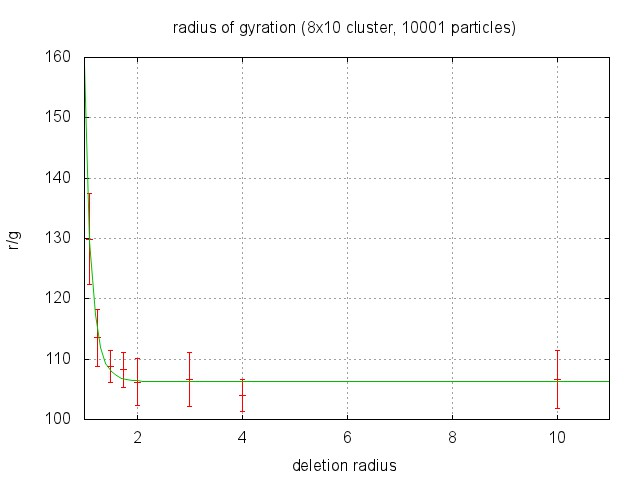
\includegraphics[width=7cm]{img/killradius.jpg}
                    \caption[The dependence of the radius of gyration on the `kill-radius']
                        {\small\textbf{The dependence of the radius of gyration on the `kill-radius'}, i.e. the distance
                        from the center of the cluster at which diffusion particles are removed. The line is a simple power
                        law and meant for illustrational purposes only.}
                    \label{fig-killradius}
                \end{figure}

            \subsubsection{Visitor Interface}
                Because we didn't want to clutter the interface of \lstinline'world' we implemented the Visitor
                pattern\cite{bib-visitor} as an entry point for both drawing and statistics facilities. In a later
                implementation the currently \lstinline'public' methods \lstinline'get_particles' and
                \lstinline'get_clusters' will disappear and will be replaced by a more versatile interface.

                We implemented real-time drawing in the beginning for debugging purposes, as it is easier to see if the
                growing works from an image than from raw data or plots. Currently only Meakin and Eden drawing are
                implemented, where the latter uses the current score of a particle to select a color from a scale.
                Because it was very difficult to see anything from the 3D renderings, we added an anaglyph drawer, which
                enabled us to see the fractal structure with red-cyan glasses. One of those renderings is seen in
                Figure~\ref{fig-anaglyph}.
                \begin{figure}
                    \center
                    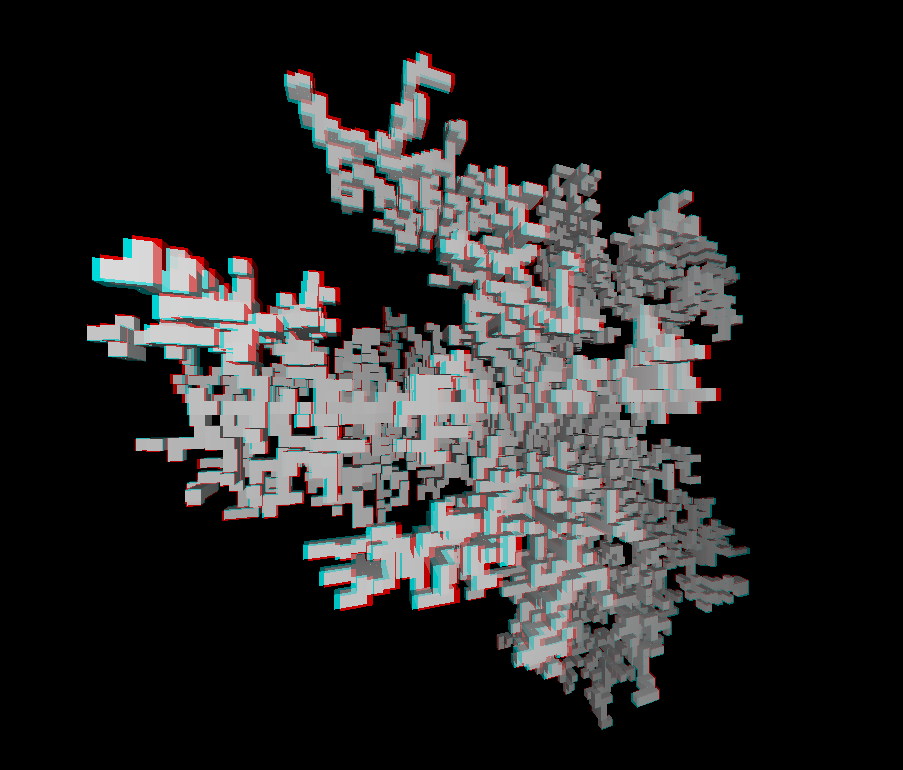
\includegraphics[width=7cm]{img/anaglyph.png}
                    \caption[An anaglyph of a 3-d Meakin cluster]
                        {\small\textbf{An anaglyph of a 3-d Meakin cluster} of 8,000 particles}
                    \label{fig-anaglyph}
                \end{figure}

                Our \lstinline'statistics_visitor' lets one plug different calculators together and outputs a header and
                data lines to a specified stream. The produced files where used for all our dimensionality calculations.

        \subsection{Examples}
           \subsubsection{Higher statistics on DLA clusters}
                Limited by the computational resources available at his time, Meakin based his conclusions about
                the properties of diffusion limited aggregation on a handful of clusters. He used those to estimate
                their fractal dimension given by the radius of gyration and the density-density-correlation in
                2- to 6-dimensional space and concluded $d\approx\frac{5}{6}D$ where $D$ is the topological, i.e. here
                also the embedding, dimension. This is only a heurestic result, e.g. you can easily see that it does
                not hold for $D=1$, where $d=1$ as well. Additionally, there are strong fluctuations in dimensionality
                even for particle numbers as large as 10,000, so there is some uncertainty left. Being unaware of any
                theoretical results for DLAs settling that issue, we checked Meakin's results on 196 clusters in
                two and three dimensions up to 100,000 particles respectively. Care was taken to reduce
                autocorrelations: all growth
                processes were uniquely seeded and entered the statistics only once, i.e. a cluster with a final
                size of 50,000 particles has not been used as a cluster of 20,000 particles at some earlier stage
                of its development. Applying the radius of gyration method to determine the clusters' dimensionality
                we obtained $d\pm\Delta d=1.70\pm0.02$ for $D=2$ and $d\pm\Delta d=2.50\pm0.03$  for $D=3$ in perfect
                accordance to Meakin's results. Determining the dimension by the density-density-correlation can
                not be automated as easily, as range in which it scales in a fractal fashion is less obvious.
                Nevertheless, it was checked by hand in about ten cases for each dimensionality giving no significant
                deviation from the values obtained via the radius of gyration, as already stated by Meakin.
                Some seven-dimensional cluster have been grown, but since dense storage soon becomes unfeasible,
                the main speed advantage of our implementation is lost. While the results required are not statistically
                significant and may suffer from finite-size artifacts, they still do not rule out the `law of $\frac{5}{6}$'.
                The large fluctuations in fractal dimensionality Meakin observed at 10,000 particles, unfortunately
                do not decrease when going to clusters of 100,000 particles. It seems likely that this is not due to
                a finite-size effect, but rather an artifact inherent in the methods of measurement (radius of gyration
                and density-density-correlation). Remember -- the structures are \emph{not} true fractals in the
                mathematical sense. Interestingly, our data cannot rule out that the fractal dimension $d$ is in fact
                a random variable with expectation value of about $\frac{5}{6}D$ even in the limit
                $N\rightarrow\infty$.

            \subsubsection{Cluster diffusion}
                Instead of growing cluster from diffusing particles, one could as well grow a cluster from diffusing
                clusters. One could take several of cluster-diffusion-grown clusters to grow a higher-order cluster
                still. One could go on like this. Where is the point? Earlier, we have seen that the fractal dimension
                of a structure is connected to its scaling behaviour. If we now compose clusters from smaller clusters
                of a given size, we impose an additional scaling behaviour onto the system. In general, the overall
                dimension will result from the original, statistically induced scaling behaviour and this new one in
                some complicated way we do not want do investigate further here. Instead, we just grow 70 clusters by the
                following recipie:
                \begin{itemize}
                    \item build a cluster of $n$ particles according to Meakin's original model
                    \item take $n$ of these cluster to assemble a new cluster
                    \item go on like this until the currently assembled cluster has more than 10,000 particles
                \end{itemize}
                Changing $n$ from 5 to 50 in increments of 5, dimensions between 1.7 and 1.3 can be created. Moreover
                $dim(n)$ appears to be monotonic. Other than just the final size, the average coordination number
                remains unchanged. So we can change the fractal dimension while maintaining other properties.
                Most important, we could stay with our original growth principle of Brownian motion and adhesion,
                which, after all, has been physically motivated.

            \subsubsection{Dendrites}
                Dendrites, as commonly found in mineralogy, are fern-like structures on rocks. They are easily confused
                with plant fossils (\emph{dendron} even is Greek for \emph{tree}) although they are entirely anorganic
                in origin. Usually, they are formed by sedimenting metal oxides. In fact, this is the very process
                which inspired Witten and Sander in the first place. The important difference to the Meakin clusters
                we have discussed so far is that in this case there is a preferred orientation. In nature, it is
                induced by the flow of water carrying the sediments (and maybe to some extend also by the geometry
                of the rock, the \emph{seed} in the language of the growth model). The Meakin model can be adapted
                to describe this process in the following straight-forward way:
                \begin{itemize}
                    \item create particles not uniformly on the n-sphere, but with a fixed $x_0$ coordinate. All other
                        coordinates can be distributed uniformly.
                    \item increase the probability for stepping along the 0-direction in the random walk. The more
                        probable it becomes, the stronger is the `flow'.
                    \item seed with a solid plane of particles perpendicular to the 0-direction not too close to where
                        particles are created.
                \end{itemize}
                Depending on the strength of the `flow', you can grow pine-like (strong) or bush-like (light) dendrites.
                The distribution of the other coordinates upon creation does not seem to have much influence as long
                as it is continuous. Otherwise, several dendrites can be grown simultaneously. The influence of the
                seeding geometry has not been studied systematically, but we conjecture that apart from determining the
                initial position of the dendrite, it has no observable effect, because as with the original Meakin model
                new particles are nearly exclusively added to the outer regions of the dendrite. Other interesting
                modifications would be the introduction of vortices in the `flow' or sticking probabilities.
                Some dendrites grown with this model at a high flow rate are displayed in fig.~\ref{fig-dendrites}.

                \begin{figure}
                    \center
                    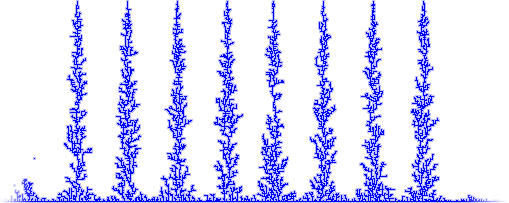
\includegraphics[width=7cm]{img/dendrites.png}
                    \caption[Dendrites as found in mineralogy]
                        {\small\textbf{Dendrites as found in mineralogy} develop if the random walk has a preferred
                        direction. This example was grown with a high flow rate, which leads to pine-shaped
                        structures.}
                    \label{fig-dendrites}
                \end{figure}

            \subsubsection{A toy model: tubes}
                The idea of preferred directions and boundary conditions can also lead to quite a different set-up:
                By the techniques developed for dendrites, you can also model particles flowing through a tube. In
                this case, an n-dimensional tube shall be a hollow n-dimensional cuboid the 0-extend of which is much
                larger than all other. The direction of flow is chosen to be the 0-direction. Depending on the size of
                the tube, the flow rate and the incoming particle density, dendrites growing from the boundaries will
                at some point block the tube entirely. This is of course hardly a useful model to describe real world
                phenoma or even useful in engineering. On can, however, learn some things about the behaviour of the
                Meakin model if many free particles are involved. One non-obvious result is that the tube will stay
                clear of obstacles for a longer time if more particles are injected. This is because the higher the
                density, the more likely it is for middle-sized clusters to form during transport. According to the
                concept of mass introduced by Meakin, the probability for those cluster to touch the tube before
                leaving it, become smaller.

            \subsubsection{Dendrites and crystals}
                %coulomb

            \subsubsection{Growing towards the sun}
                This final example is based on the Eden-Meakin model. Again, the basic idea is to introduce a preferred
                direction. Additionally, as we know of the adaptive nature of this particular model, we shall try to
                change the preferred direction over time. For the sake of concreteness let us attempt to model a plant
                growing towards to sun. We will try to do so by only changing the scoring algorithm. The creation of
                new particles shall still be possible at each nearest-neighbour site. That way, we want to emulate to
                process of natural selection on a microbiologic level. In altering the scoring procedure we have to take
                care not to create a situation in which a particle has a higher score than any of its ancestors because
                we do not want the cluster to be split. This leaves only a limited number of possibilities one of which
                is to introduce an additional factor for the chain score, such that $\Delta S=\gamma(\vec x)/(1+l)^\eta$,
                where $\vec x$ is the position of the new particle. Since our new scoring should somehow reflect the
                influence of the sun, seed the cluster at the origin and choose
                
                \begin{equation*}
                    \gamma(\vec x)=
                    \begin{cases}
                            \frac{\vec x\cdot \hat s}{|x|}  & \text{if $x_0>0$} \\
                            0 & \text{if $x_0\le 0$},
                    \end{cases}
                \end{equation*}

                where $\hat s$ is a unit-vector pointing into the direction of the sun. This reflects the fact
                that sunlight reaches the earth essentially as parallel rays. The 0-direction is
                interpreted as the `up-direction'. It is known that the growth
                of plants is also crucially influenced by the direction of gravity, but we shall neglect that here
                and forbid growth downwards manually.

                Fig.~\ref{fig-edentree} depicts in 2 dimensions the extreme case, where the sun has been situated
                at $(0,1)$ during the first 10,000 steps and at $(0, -1)$ afterwards. It can clearly be seen, how
                the plant follows the sun. The `old' branches gradually degenerate because the sun never returns.

                In a more sophisticated model, where the sun moves continuously, one encounters the following
                behaviour: depending on the rate of growth determined by the parameters $\eta$ and $N_m$, the
                plant follows the sun for a few `days'. At some point however, the memory effect described before
                inhibits a timely adaptation and the plant only `sees' the average illumination becoming
                symmetric and time-invariant in the upper half-space. As with the original Eden-Meakin-model, a
                stationary phase is reached. There also is another possible outcome: if the `night' is too long,
                the plant may `die', i.e. a particles are removed. Again, due to the memory effect this will
                only happen during the first night or not at all.

                Instead of only talking about living and dying plants, one could now implement some kind of
                scoring for a plant as a whole, describing its adaptivity with respect to environmental constraints.
                Together with an enlarged parameter set for the clusters, being determined by some genetic
                algorithm based on this scoring, one would obtain a toy-model of evolution.

                While this is in a direct line with Eden's original aims, we are now admittedly abandoning
                the realm of fractal growth -- and so the scope of this text.

        {\small
            \paragraph{Further reading}
            Again, Meakin's results on DLA are summarized in \cite{src-meakin1}. The Eden-Meakin model is based
            on \cite{src-eden} and \cite{src-meakin-eden}.
            A development version of \texttt{trivial} can freely be obtained from \texttt{github.com} as the
            repository \texttt{comp\_phys} of \emph{filmor}'s. Please note that at the time of writing, it is still
            heavily under construction and some parts may not be functional or only implemented in a `hackish' way.
        }

        \begin{figure}
            \center
            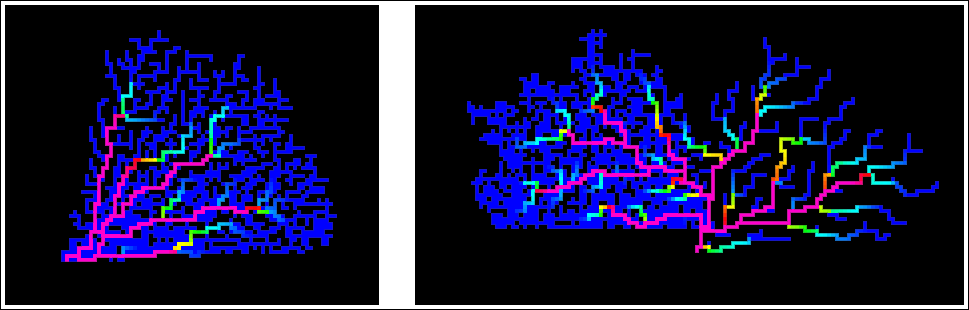
\includegraphics[width=8cm]{img/edentree.png}
            \caption[A tree]
                {\small\textbf{A tree} is what one might see in this particularly scored Eden model. During
                the first 10,000 steps, the direction of the sun is $\hat s=(0,1)$ and $\hat s=(0,-1)$ later
                (text).}
            \label{fig-edentree}
        \end{figure}


        \subsection{Limits of the Current Approach and Outlook}
            \label{sec-limits}
            The current implementation has some drawbacks and unattractivenesses. A main problem are the
            interactions. For starters it is very complicated to implement additional interactions, like the Coulomb
            interaction. One has overload \lstinline'interact' three times with nearly identical code, which is
            quite unfortunate. It should also maybe renamed to \lstinline'interact_with', because it handles the
            interaction of the first object with the second and is not symmetric.

            A major drawback of our current approach is that we can't define different boundaries for clusters. This
            would be very favorable for example for the Dendrites, because their natural boundary is not a sphere but
            rather the current height of the crystals. Also the tube model could be sped up with that.

            To make the code less error-prone it would also be good to unify the interfaces of clusters and particles
            somehow, because the code of \lstinline'world::step' is currently very repetitive and one has to see if
            \lstinline'position' or \lstinline'get_center()' has to be used. Also it is unpleasant that particles play
            a dual role, as carriers of charge or other interaction information on the one hand, which the also have
            when contained in clusters, and as a kind of "`single-particle clusters"' on the other, which they only
            have as free particles.

            To tackle all theses problems we're trying to define new, more general concepts. We will introduce concept
            \lstinline'ParticleContainer' which roughly covers \lstinline'static_cluster' and
            \lstinline'single_particle'. All bounding calculations are to be done inside the object itself. Furthermore
            we will introduce \lstinline'Interaction', which defines all particle-state information (which is the
            \lstinline'value_type' of \lstinline'ParticleContainer') and is chainable, so that we can for example add
            an electric charge to sticky particles.

            This will enable us to streamline great amounts of our code and see how the fractals change when
            interactions are turned on.

    \section{Conclusion}
        Even 30 years after its advent, fractal growth still is an exciting topic and not completely unterstood.
        There are many links to other disciplines besides mathematics and physics, be it biology, engineering,
        computer science or art.

        In fact, there is one additional striking feature about fractals in general: They are considered beautiful. We
        have seen that there is a deep connection between dimensionality and scaling laws, i.e. self-similarity. The
        question whether the perceived beauty of fractals is due to this special kind of symmetry (the human brain
        seeming to react to symmetry on a very fundamental level), or the perceived beauty of symmetries is due to
        fractals being a phenomenon common in nature remains for the reader to solve or maybe psychology.

    \begin{thebibliography}{99}
        \bibitem{src-wittensander} T. A. Witten and L. M. Sander, Phys. Rev. Lett. 47, 1400 (1981)
        \bibitem{src-stanley} H. E. Stanley, J. Phys. A 10, L211 (1977)
        \bibitem{src-meakin1} P. Meakin, Phys. Rev. A 27, 1495 (1983)
        \bibitem{src-meakin2} P. Meakin, Phys. Rev. Lett. 51, 13 (1983)
        \bibitem{src-eden} M. Eden, Proc. 4th Berkeley Symp. on Mathematics, Statistics and Probability, vol. 4,
            F. Neyman, ed., (1961)
        \bibitem{src-meakin-eden} P. Meakin, Physica A, 179 (1991)
        \bibitem{src-mandelbrot} B. Mandelbrot, The Fractal Geometry of Nature, Benoit B. Mandelbrot
        \bibitem{src-matsumoto}M. Matsumoto, T. Nishimura, Mersenne twister. In: ACM Transactions on Modeling and
          Computer Simulation. 8, 1998
    \end{thebibliography}
\end{document}
